\documentclass[11pt]{article}
\usepackage[utf8]{inputenc}
\usepackage[top=60pt, bottom=60pt, left=70pt, right=70pt]{geometry}
\usepackage{graphicx}
% Default fixed font does not support bold face
\DeclareFixedFont{\ttb}{T1}{txtt}{bx}{n}{8} % for bold
\DeclareFixedFont{\ttm}{T1}{txtt}{m}{n}{8}  % for normal

\title{Code Overview}
\author{Daniel W. Zaide}

\begin{document}

\maketitle

\section{Overview}

This code was developed to model facade envelopes with several main objectives:
\begin{itemize}
\item Versatility - The code should be versatile, flexible, and handle a wide range of possible physics
\item Simplicity - The code should be simple, and defining new components and physics should be easy and clean
\item Readable - Outside of the infrastructure, the physics components and problem setup should be readable
\end{itemize}

With that in mind, we leverage python using {\bf list} and {\bf dict}, rather than numerical arrays to allow for flexibility. We also use function handles to allow for easy definition of functions and allow for runtime adding variables classes.

There are five main files in the base, {\bf src/base}, directory:
\begin{itemize}
\item [blocks.py] - contains definitions of block objects, our control volume like object
\item [flux.py] - contains definitions of fluxes and flux functions
\item [source.py] - contains definitions of sources and source functions
\item [problem.py] - contains solvers, manages system construction
\item [geom.py] - contains geometry specifically for facade simulations
\end{itemize}
\section{Infrastructure of base directory}
The goal is ultimately to solve the global system
\begin{equation}
\mathbf{R}(\mathbf{U}) = \sum_F \mathbf{F}(\mathbf{U}) + \sum_S \mathbf{S}(\mathbf{U}) = \mathbf{0}
\end{equation}
for a set of states $\mathbf{U}$, flux functions $\mathbf{F}$, and sources $\mathbf{S}$. Rather than a typical control volume approach, a simpler abstraction is used: {\bf blocks}. Each block has its own state variables, and the equations for these state variables are defined by fluxes (information from neighboring blocks) and sources (external information). Boundary conditions are done implicitly with a ghost cell type approach, defining blocks with states that remain constant. Wrapping the whole thing together is a {\bf problem} object, which is initialized with the blocks we are solving for. The boundary blocks are created, but are passed in separately to the problem object.

\subsection{Blocks}
Each typical control volume can be considered as a block. Blocks are connected to other blocks through fluxes, which act as boundary conditions. Blocks can have arbitrary state variables, and not all blocks have to have the same set of states, provided flux functions are defined that connect them together. Every block has a set of states, $U$, stored in the {\bf .state}. Consider a block with temperature, density, and velocity defined. The state for example, may look like
\begin{verbatim}
>>> block.state
OrderedDict([('T',20), ('rho',1.05), ('u',0.01)])
\end{verbatim}
where the ordered dictionary is used to preserve the mapping used in construction of the global problem. We can access these variables using the dict, such as {\bf block.state['T']}. Every block defines its own equation
\begin{equation}
R(U) = \sum_{(F,N)} F(U,N) + \sum_S S(U) = 0
\end{equation}
for block $B$, its states $U \in B$, and its connected neighboring blocks, $N$ and corresponding fluxes. In this framework the {\bf OrderedDict} structure is used to keep track of state variables. Each block can have its own set of states, provided there is an equation (flux or source) to be solved (R cannot be empty). The form of this will be a dictionary, and the sum of the fluxes and sources will be a sum over similar dictionaries.

Blocks contain additional information, such as materials or constant properties in the form of dictionaries of functions and function parameters. These are defined at initialization. This is implemented and documented in {\bf blocks.py}
\subsection{Fluxes}
Fluxes are defined through blocks which remain constant, such as external temperatures or inflow conditions. Each flux is a function of two blocks, the block they belong to, and their neighboring block. Boundary conditions are currently defined by fluxes with one block not part of the problem (constant). Each flux function is defined in {\bf flux.py}, and is initialized by passing in the flux function name. Fluxes are one directional (from one block to another) and are assigned to a block, using the {\bf addFlux} function for a block. Flux functions also contain their own parameters, a dictionary of constants they can use.
\subsection{Sources}
Sources are defined similar to fluxes, but are functions of a block. They are defined in {\bf source.py}.
\subsection{Problem}
This is a class that serves as a wrapper for everything, converting from the local block regions into a global matrix and back to do the solve. The problem is initialized with a list of blocks.
\begin{verbatim}
def __init__(self,blocks):
		self.b = blocks
		self.mapping = [(i, k) for i, b in enumerate(blocks) for k in b.state.keys()]
\end{verbatim}
where the mapping between blocks into a global list is done at initialization, and stored for reuse. 
\begin{verbatim}
def solve(self):
		solution = [None]*len(self.mapping)
		for ix, (i,k) in enumerate(self.mapping):
			solution[ix] = self.b[i].state[k]
		solution = fsolve(self.r, solution)
		self.update(solution)
\end{verbatim}
This class is the one that needs the least work, the only places that should be modified are in {\bf solution = fsolve(self.r, solution)}, where {\bf fsolve} is a built-in function from {\bf scipy.optimize}.

There is also an unsteady solve which solves time-dependent ODEs using {\bf scipy.odeint}, see diffusion2D.py for an example.

\subsection{Geometry}

Geometry is defined in text files (see data/geometry/whole-building.txt) and is implemented and described in src/base/geom.py. Given a geometry file consisting of coordinates forming quadrilateral surfaces, e.g., the snippet shown below,
\begin{verbatim}
{25.965603, -16.047859, 0.5}
{25.964993, -16.047247, 4.0}
{-25.964993, -16.047247, 4.0}
{-25.964993, -16.047859, 0.5}
{25.965603, 16.047859, 0.5}
{25.964993, 16.047247, 4.0}
{25.964993, -16.047247, 4.0}
{25.965603, -16.047859, 0.5}
...
\end{verbatim}
a quadrilateral can be expressed by its four vertices as $Q = [\mathbf{v}_0,\mathbf{v}_1,\mathbf{v}_2,\mathbf{v}_3]$. The quadrilateral lies in a plane represented by a normal vector, $\mathbf{n} = [n_x,n_y,n_z]$, which can be computed from any three points as 
\[
\mathbf{n} = S(\mathbf{v}_2-\mathbf{v}_0)\times (\mathbf{v}_1-\mathbf{v}_0)
\]
where the sign, $S = \pm 1$, of the vector is chosen to ensure the normal vector points outward, with $S = -1$ for walls and $S = 1$ for the roof. This is as a result of the vertex ordering. The vertex ordering is shown in figure \ref{fig:ordering}

\begin{figure}
\centering
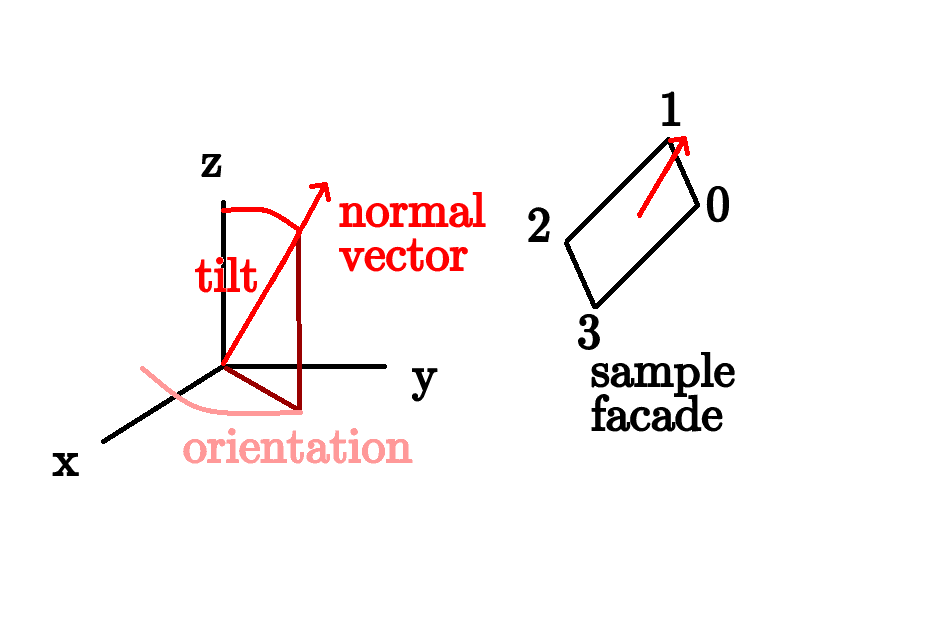
\includegraphics[width=0.75\textwidth]{images/geomdefine2.png}
\caption{Vertex Ordering}
\label{fig:ordering}
\end{figure}
The normal vectors for the example file are plotted in Figure \ref{fig:normals}.
\begin{figure}
\centering
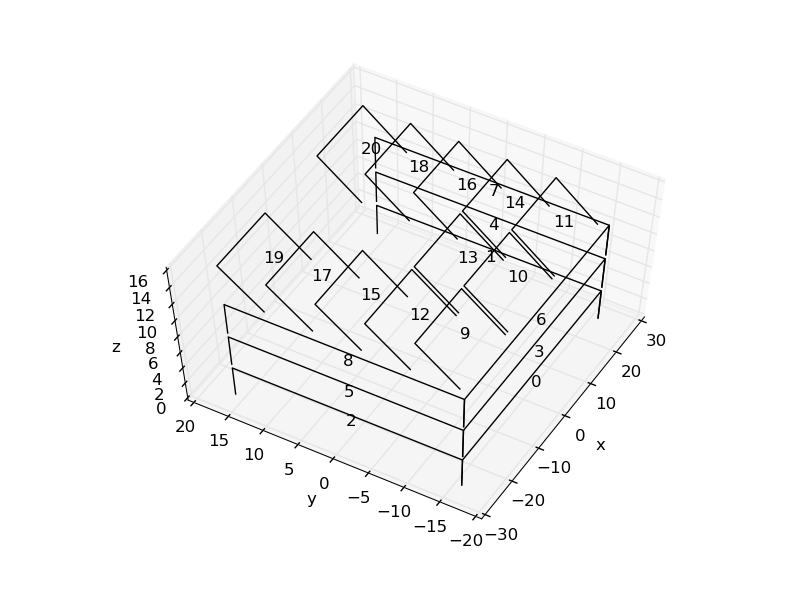
\includegraphics[width=1.0\textwidth]{images/whole-building.png}
\caption{Normal Vectors}
\label{fig:normals}
\end{figure}
From the normal vectors, the orientation of the quadrilateral surface(with respect to latitude/longitude) can be written as
\[
\theta_{orientation} = \tan^{-1}\frac{n_y}{n_x}
\]
and the tilt (with respect to the x-y plane) is
\[
\theta_{tilt} = 90^\circ - \tan^{-1}\frac{\sqrt{n_x^2+n_y^2}}{n_z}
\]

The pitch and yaw of the quadrilateral can then be computed from the time, orientation, tilt, latitude, and longitude of the geometry.

Based on the ordering of the vertices, the width and height are 
\[ w = ||\mathbf{v}_2-\mathbf{v}_1||, \qquad h = ||\mathbf{v}_1-\mathbf{v}_0||
\]
and the number of modules for a given surface are 
\[
n_{horizontal} = floor(w/w_{module}), \qquad n_{vertical} = floor(h/h_{module})
\]
for some chosen module dimensions. Choosing $w_{module} = h_{module} = 0.33$ gives the following setup with, the walls being either 97x10 or 157x10, and the roof panels being 13x8.

\begin{figure}
\centering
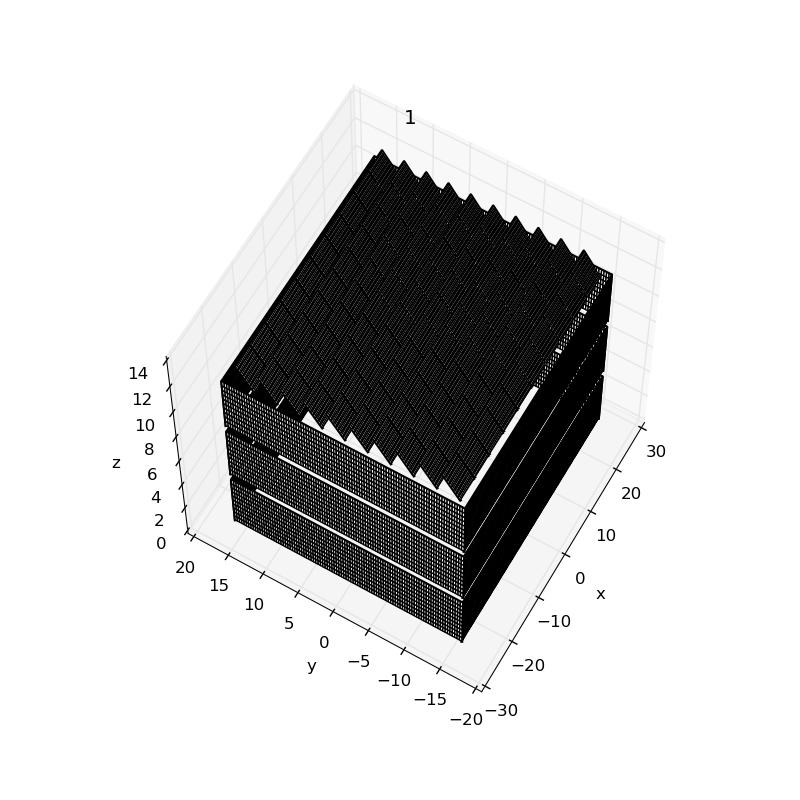
\includegraphics[width=1.0\textwidth]{images/whole-building-all.png}
\caption{Geometry, with modules drawn in as squares.}
\label{fig:normals}
\end{figure}
\section{Other Files}
The main support files are in the {\bf src} directory.
\begin{itemize}
\item casegeom.py, geometry readers and writers, geometry creation
\item icsolar.py, main icsolar solver, contains the model (see the publication for math)
\item solar.py, solar calculations 
\item icsolar\_support.py, support functions, such as material definitions
\item shading.py, shading calculations
\item weather.py, readers for TMY data
\end{itemize}

The are also other files for a drips model and some uncertainty quantification using the DAKOTA software. \\

The main programs for ICSolar are {\bf ICSolar.py}, containing the whole-building model and {\bf ICSolar\_Validation.py}, which runs the validation of the model with experimental data in the {\bf data} directory. All results are in a directory, {\bf Results} which will be created. There is also a {\bf ICSolar\_Dakota.py}, which does uncertainty quantification, and a {\bf Drips.py}, which does the model described in drips.tex.
\end{document}
